% Glava dokumenta
\documentclass{beamer}
\usepackage[slovene]{babel}
\usepackage[utf8]{inputenc}
\usepackage{lmodern}
\usepackage[T1]{fontenc}
\usepackage{amsthm}
\usepackage{amsmath}
\usepackage{listings}
\usepackage{amssymb}
\usepackage{graphicx}
\usepackage{url}
\usepackage{multirow}
\usetheme{Warsaw}
\setbeamercovered{transparent}
%\usecolortheme{crane}
\title[Verjetnost prekomernega prileganja]{VERJETNOST PREKOMERNEGA PRILEGANJA}
\author[Tina Janša]{Tina Janša}


\begin{document}


\begin{frame}
\titlepage
\end{frame}


\begin{frame}
\frametitle{Uvod}

%\begin{block}{Naloga}
%Za dani nabor trgovalnih strategij izračunaj verjetnost prekomernega prileganja z novo metodo kombinatoričnega simetričnega prečnega preverjanja.
%\end{block}
%\vspace{0.5cm}
\begin{itemize}
\item Obdelava podatkov \pause
\item Implementacija trgovalnih strategij 
\item Implementacija metode kombinatoričnega simetričnega prečnega preverjanja
\end{itemize}

\end{frame}


%\begin{frame}
%\frametitle{Podatki}
%S\&P 500 - borzni indeks, ki temelji na tržni kapitalizaciji 500 velikih podjetji, katerih navadne delnice kotirajo na Newyorški borzi ali NASDAQ
%\end{frame}

\begin{frame}
\frametitle{Trgovalne strategije}
\begin{itemize}
\item Random
\item Buy \& Hold
\item SMA
\item RSI
\item Bollinger
\end{itemize}
\end{frame}


\begin{frame}
\frametitle{SMA - Preprosto drseče povprečje}
\begin{itemize}
\item Nakupni signal: zadnja cena > SMA
\item Prodajni signal: zadnja cena < SMA
\end{itemize}

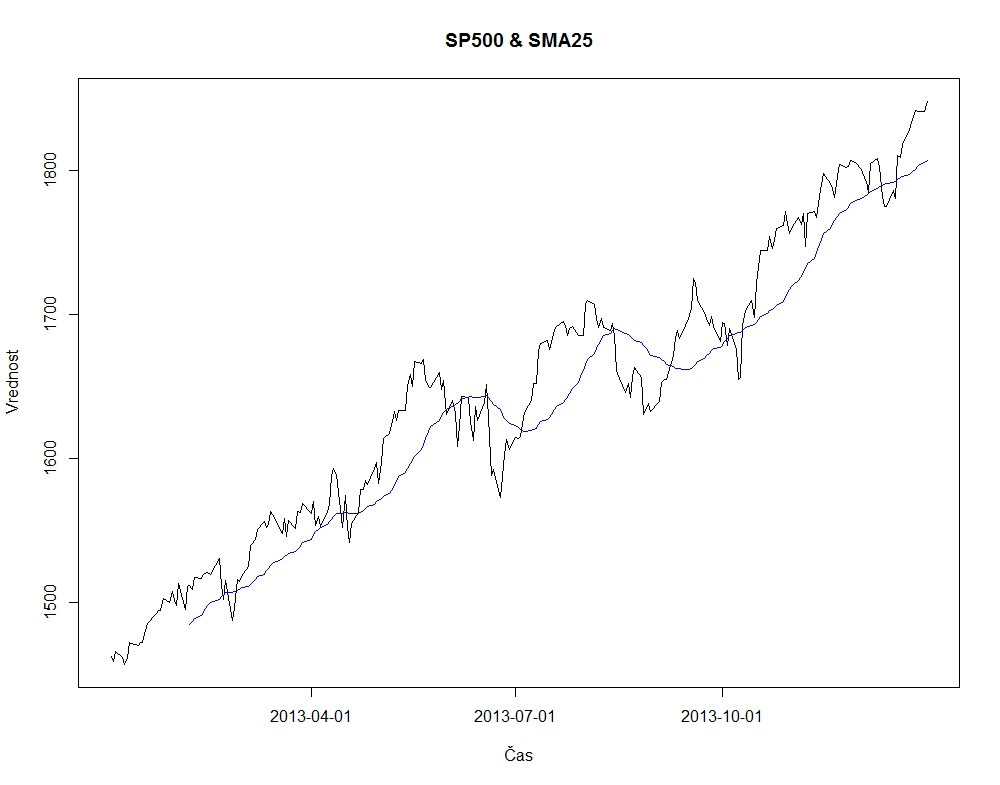
\includegraphics[width=10cm]{SMA25.png}

\end{frame}


%\begin{frame}
%\frametitle{RSI - Indeks relativne moči}
%\begin{columns}
%\begin{column}{5cm}
%\begin{itemize}
%\item Nakupni signal: RSI < 30
%\item Prodajni signal: RSI > 70
%\end{itemize}
%
%$$RSI = 100 - \frac{100}{1-RS}$$
%
%\end{column}
%
%\begin{column}{6.3cm}
%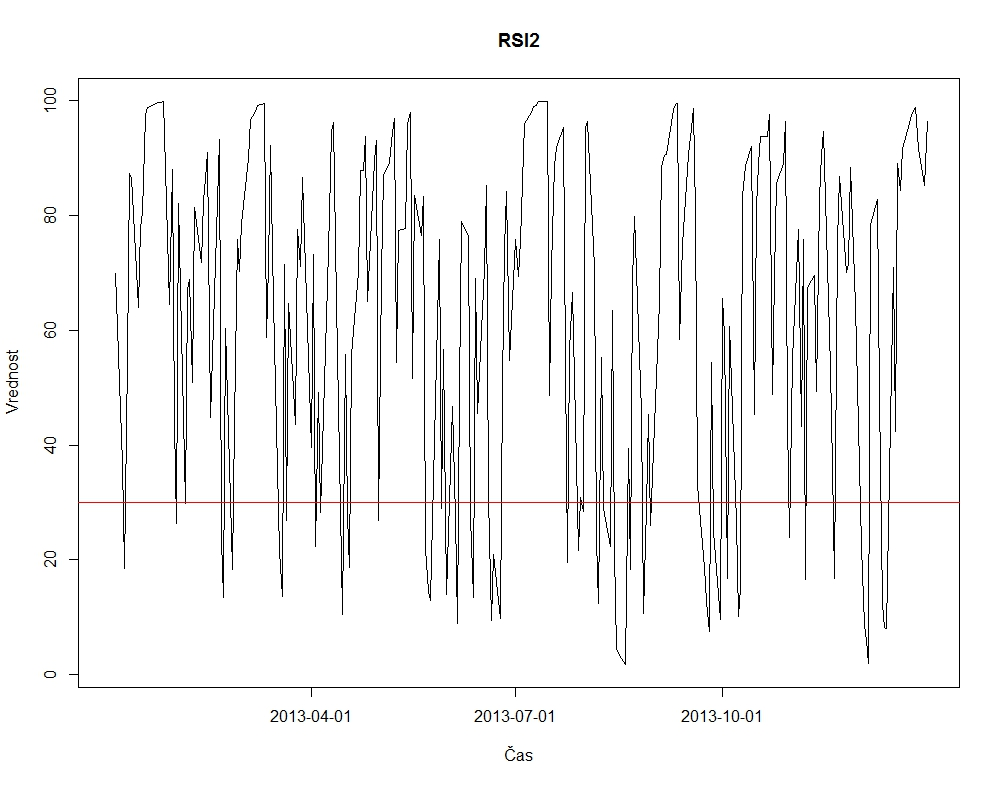
\includegraphics[width=6.3cm]{RSI2.png}
%\end{column}
%\end{columns}
%\vspace{0.5cm}
%$$RS = \frac{\textrm{povprečna vrednost pozitivnih period}}{\textrm{povprečna vrednost negativnih period}}$$
%\end{frame}

\begin{frame}
\frametitle{RSI - Indeks relativne moči}
\begin{itemize}
\item Nakupni signal: RSI < 30
\item Prodajni signal: RSI > 70
\end{itemize}

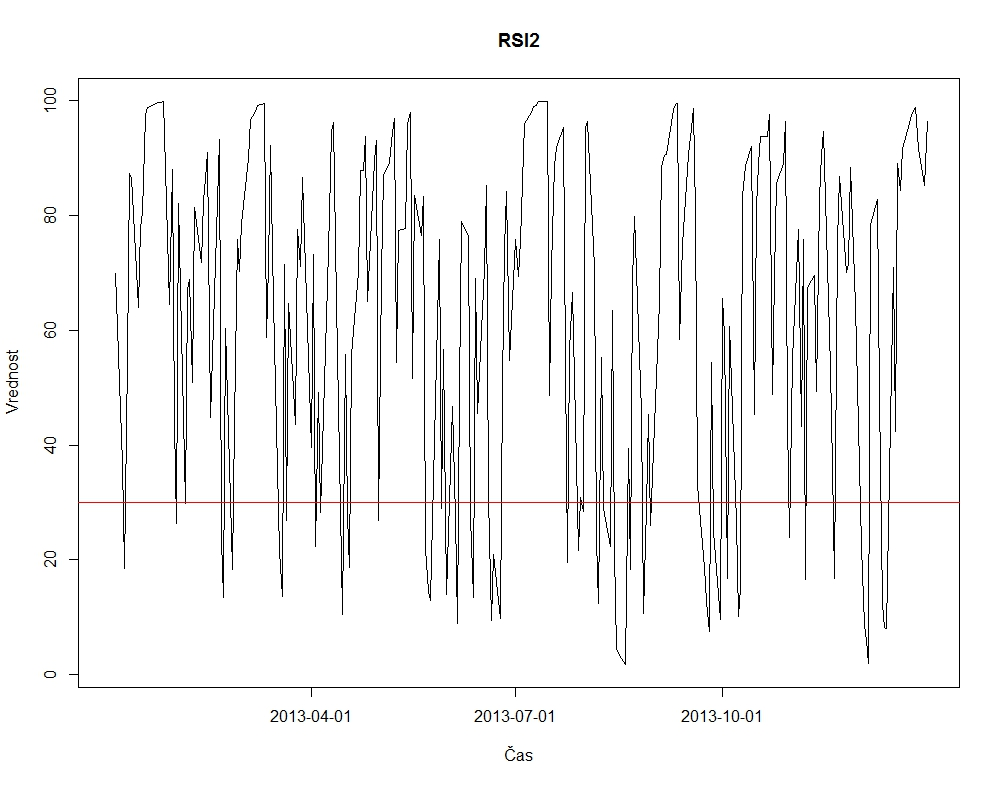
\includegraphics[width=10cm]{RSI2.png}

\end{frame}


\begin{frame}
\frametitle{Bollingerjevi pasovi}
\begin{itemize}
\item Nakupni signal: zadnja cena < spodnji pas
\item Prodajni signal: zadnja cena > zgornji pas
\end{itemize}
\begin{itemize}
\item zgornji pas = SMA + faktor $\times$ standardni odklon
\item srednji pas = SMA
\item spodnji pas = SMA - faktor $\times$ standardni odklon
\end{itemize}
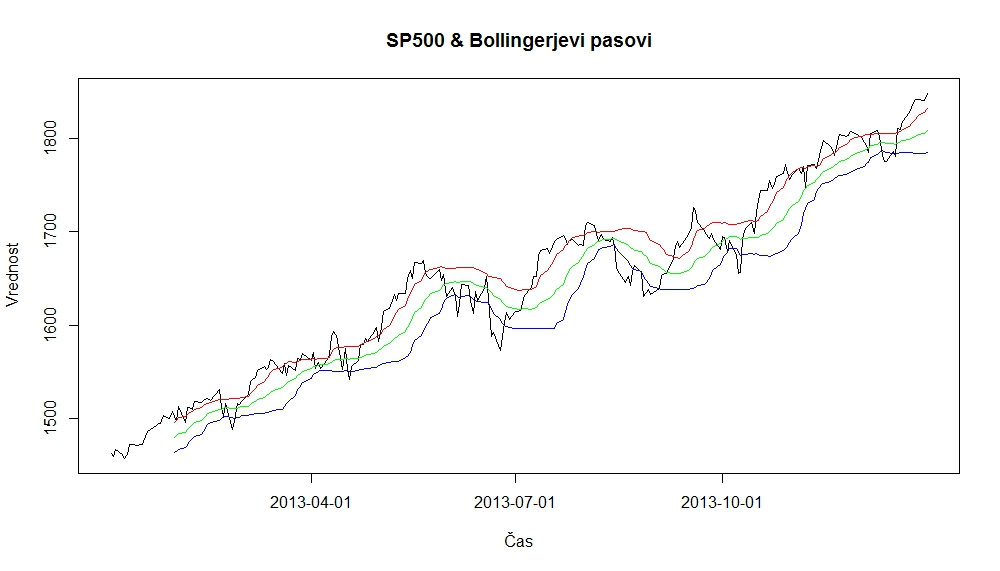
\includegraphics[width=10cm]{Bollinger.png}

\end{frame}


\begin{frame}
\frametitle{Trgovalne strategije}
\includegraphics[width=11cm]{kapital_5let.png}
\end{frame}

\begin{frame}
\frametitle{Prekomerno prileganje}
\begin{itemize}
\item Sharpovo razmerje: mera uspešnosti strategije ($\frac{\mu}{\sigma}$) \pause
\item Prekomerno prileganje: Naj bo n najboljša strategija na učni množici. Proces izbire strategije se prekomerno prilega, če za strategijo n velja, da je njena pričakovana uspešnost na testni množici manjša od mediane uspešnosti vseh strategij na testni množici.
\pause
\item Verjetnost prekomernega prileganja je verjetnost, da je uspešnost strategije n na testni množici manjša od mediane uspešnosti vseh strategij na testni množici. 
\end{itemize}
\end{frame}


\begin{frame}
\frametitle{Metoda kombinatoričnega simetričnega prečnega preverjanja}
\begin{itemize}
\item	Dnevni donosi portfelja za N strategij na obdobju dolžine T. 
\item	Razdelimo na S enako dolgih podobdobij.
\item	Podobdobja razdelimo na učno in testno množico. 
\item	Določimo uspešnost strategij na učni in testni množici.
\item	Za strategijo, ki je najboljša na učni množici (n) določimo relativno uspešnost na testni množici - $\omega \in (0,1)$. 
\item	Definiramo $\lambda = log\frac{\omega}{1-\omega}$
\item	Frekvenčna porazdelitev $\lambda$.
\item Verjetnost prekomernega prileganja je frekvenca negativnih $\lambda$. Označimo jo z $\Phi$.
\end{itemize}
\end{frame}

\begin{frame}
\frametitle{Metoda kombinatoričnega simetričnega prečnega preverjanja}
\begin{itemize}
\item $\Phi \approx 0$: ni velikega prekomernega prileganja, izbor optimalne strategije na učni množici pripomore k večji uspešnosti na testni množici.
\item $\Phi = \frac{1}{2}$: zgodovinsko preverjanje se prekomerno prilega do te mere, da postopek izbora optimalne strategije na učni množici ne doda vrednosti.
\item $\Phi >> \frac{1}{2}$: prekomerno prileganje je tako veliko, da izbor optimalne strategije na učni množici povzroči slabšo pričakovano uspešnost na testni množici, kot bi bila, če bi naključno izbrali eno izmed strategij.
\end{itemize}

\end{frame}


%\begin{frame}
%\frametitle{Rezultati}
%{\footnotesize
%\begin{tabular}{|p{1.15cm}|p{0.8cm}|p{1.4cm}|p{1.4cm}|p{1.2cm}|p{1.2cm}|p{1.2cm}|}
%\cline{3-7}
%\multicolumn{2}{c|}{}&\multicolumn{5}{|c|}{\textbf{STRATEGIJE}}\\
%\cline{3-7}
%\multicolumn{2}{c|}{} & SMA150 & SMA150 & RSI2 & RSI2 & \multirow{5}{1cm}{vse strategije} \\
%\multicolumn{2}{c|}{} & RSI14 & RSI14 & Bollinger & Bollinger & \\
%\multicolumn{2}{c|}{} & Buy\&Hold &  Buy\&Hold  & Random & Random & \\
%\multicolumn{2}{c|}{} & & SMA50 & & SMA25 & \\
%\multicolumn{2}{c|}{} & & Random &   & RSI14 &  \\
%\hline
%\multirow{2}{*}{\textbf{CSCV}} & 5 let & 0.7953 & 0.8038 & 0.0004 & 0.0026 & 0.1060 \\
% & 13 let & 0.7416 & 0.7025 & 0.0017 & 0.0039 & 0.0333 \\
%\hline
%\multirow{2}{*}{\textbf{Hold-out}} & 5 let & 3 & 5 & 3 & 5 & vse \\
% & 13 let & 3 & 5 & 3 & 5 & vse \\
% \hline
%\end{tabular}
%}
%\end{frame}

\begin{frame}
\frametitle{Rezultati}
\begin{tabular}{|c|c|c|c|c|p{1.2cm}|}
\hline
\multirow{5}{*}{} & SMA150 & SMA150 & RSI2 & RSI2 & \multirow{5}{1.2cm}{vseh 9 strategij} \\
& RSI14 & RSI14 & Bollinger & Bollinger & \\
& Buy\&Hold &  Buy\&Hold  & Random & Random & \\
& & SMA50 & & SMA25 & \\
& & Random &   & RSI14 &  \\
\hline
PBO & 0.7953 & 0.8038 & 0.0004 & 0.0026 & 0.1060 \\
 \hline
\end{tabular}
\end{frame}



\begin{frame}
\includegraphics[width=11cm]{velik_overfit_3strategije_5let.png}
\end{frame}

\begin{frame}
\includegraphics[width=11cm]{velik_overfit_5strategij_5let.png}
\end{frame}

%\begin{frame}
%\includegraphics[width=11cm]{velik_overfit_3strategije_13let.png}
%\end{frame}

%\begin{frame}
%\includegraphics[width=11cm]{velik_overfit_5strategij_13let.png}
%\end{frame}

\begin{frame}
\includegraphics[width=11cm]{majhen_overfit_3strategije_5let.png}
\end{frame}

\begin{frame}
\includegraphics[width=11cm]{majhen_overfit_5strategij_5let.png}
\end{frame}

%\begin{frame}
%\includegraphics[width=11cm]{majhen_overfit_3strategije_13let.png}
%\end{frame}

%\begin{frame}
%\includegraphics[width=11cm]{majhen_overfit_5strategij_13let.png}
%\end{frame}

\begin{frame}
\includegraphics[width=11cm]{kapital_5let.png}
\end{frame}

%\begin{frame}
%\includegraphics[width=11cm]{kapital_13let.png}
%\end{frame}




\end{document} 
